\documentclass[11pt,twoside,a4paper]{book}
\usepackage[utf8]{inputenc}
\usepackage[T1]{fontenc}
\usepackage{latexsym}

\usepackage[brazil,brazilian]{babel}
\usepackage[pdftex]{graphicx}           
\usepackage{setspace}                   
\usepackage{indentfirst}                
\usepackage{makeidx}                  
\usepackage[nottoc]{tocbibind}     
\usepackage{courier}                    
\usepackage{type1cm}              
\usepackage{listings}                   
\usepackage{titletoc}
\usepackage{amsmath}
\usepackage[fixlanguage]{babelbib}
\usepackage[font=small,format=plain,labelfont=bf,up,textfont=it,up]{caption}
\usepackage[usenames,svgnames,dvipsnames]{xcolor}
\usepackage[a4paper,top=2.54cm,bottom=2.0cm,left=2.0cm,right=2.54cm]{geometry} % margens
\usepackage[pdftex,plainpages=false,pdfpagelabels,pagebackref,colorlinks=true,citecolor=DarkGreen,linkcolor=NavyBlue,urlcolor=DarkRed,filecolor=green,bookmarksopen=true]{hyperref} % links coloridos
\usepackage[all]{hypcap}                % soluciona o problema com o hyperref e capitulos
\usepackage[square,sort,nonamebreak,comma]{natbib}  
% \usepackage[chapter]{algorithm}
% \usepackage{algpseudocode}
\usepackage[algochapter,boxruled,linesnumbered,portuguese]{algorithm2e}
\fontsize{60}{62}\usefont{OT1}{cmr}{m}{n}{\selectfont}
\usepackage{fancyhdr}
\pagestyle{fancy}
\fancyhf{}
\renewcommand{\chaptermark}[1]{\markboth{\MakeUppercase{#1}}{}}
\renewcommand{\sectionmark}[1]{\markright{\MakeUppercase{#1}}{}}
\renewcommand{\headrulewidth}{0pt}
\renewcommand*{\lstlistingname}{Listagem}
%\renewcommand*{\lstlistoflistingname}{Lista de Listagens}
\graphicspath{{imagens/}}             
\frenchspacing                          
\urlstyle{same}                         
\makeindex                              
\raggedbottom                           
\fontsize{60}{62}\usefont{OT1}{cmr}{m}{n}{\selectfont}
\cleardoublepage
\normalsize
% Ref: http://en.wikibooks.org/wiki/LaTeX/Packages/Listings
\lstset{ %
language=Java,                  % choose the language of the code
basicstyle=\footnotesize,       % the size of the fonts that are used for the code
numbers=left,                   % where to put the line-numbers
numberstyle=\footnotesize,      % the size of the fonts that are used for the line-numbers
stepnumber=1,                   % the step between two line-numbers. If it's 1 each line will be numbered
numbersep=5pt,                  % how far the line-numbers are from the code
showspaces=false,               % show spaces adding particular underscores
showstringspaces=false,         % underline spaces within strings
showtabs=false,                 % show tabs within strings adding particular underscores
frame=single,	                % adds a frame around the code
framerule=0.6pt,
tabsize=2,	                    % sets default tabsize to 2 spaces
captionpos=b,                   % sets the caption-position to bottom
breaklines=true,                % sets automatic line breaking
breakatwhitespace=false,        % sets if automatic breaks should only happen at whitespace
escapeinside={\%*}{*)},         % if you want to add a comment within your code
backgroundcolor=\color[rgb]{1.0,1.0,1.0}, % choose the background color.
rulecolor=\color[rgb]{0.8,0.8,0.8},
extendedchars=true,
xleftmargin=10pt,
xrightmargin=10pt,
framexleftmargin=10pt,
framexrightmargin=10pt
}

% Corpo do texto
\begin{document}
\frontmatter 
\fancyhead[RO]{{\footnotesize\rightmark}\hspace{2em}\thepage}
\setcounter{tocdepth}{2}
\fancyhead[LE]{\thepage\hspace{2em}\footnotesize{\leftmark}}
\fancyhead[RE,LO]{}
\fancyhead[RO]{{\footnotesize\rightmark}\hspace{2em}\thepage}

\onehalfspacing

% ---------------------------------------------------------------------------- %
% CAPA
% Nota: O título para as dissertações/teses do IME-USP devem caber em um 
% orifício de 10,7cm de largura x 6,0cm de altura que há na capa fornecida pela SPG.
\thispagestyle{empty}
\begin{center}
    \vspace*{2.3cm}
    \textbf{\Large{Uma infraestrutura para desenvolvimento de aplicações distribuídas baseada em minitransações}}\\
    
    \vspace*{1.2cm}
    \Large{Leandro Ferro Luzia}
    
    \vskip 2cm
    \textsc{
    Dissertação apresentada\\[-0.25cm] 
    ao\\[-0.25cm]
    Instituto de Matemática e Estatística\\[-0.25cm]
    da\\[-0.25cm]
    Universidade de São Paulo\\[-0.25cm]
    para\\[-0.25cm]
    obtenção do título\\[-0.25cm]
    de\\[-0.25cm]
    Mestre em Ciências}
    
    \vskip 1.5cm
    Programa: Ciências da Computação\\
    Orientador: Prof. Dr. Francisco C. R. Reverbel
    \vskip 1cm
    
    \vskip 0.5cm
    \normalsize{São Paulo, Junho de 2013}
\end{center}

% ---------------------------------------------------------------------------- %
% Página de rosto (SÓ PARA A VERSÃO DEPOSITADA - ANTES DA DEFESA)
% Resolução CoPGr 5890 (20/12/2010)
\newpage
\thispagestyle{empty}
    \begin{center}
        \vspace*{2.3 cm}
        \textbf{\Large{Uma infraestrutura para desenvolvimento de aplicações distribuídas baseada em minitransações}}\\
        \vspace*{2 cm}
    \end{center}

    \vskip 2cm

    \begin{flushright}
	Esta é a versão original da dissertação elaborada pelo\\
	candidato Leandro Ferro Luzia, tal como \\
	submetida à Comissão Julgadora.
    \end{flushright}

\pagebreak

\pagenumbering{roman}

%\chapter*{Agradecimentos}
%Texto texto texto texto texto texto texto texto texto texto texto texto texto
%texto texto texto texto texto texto texto texto texto texto texto texto texto
%texto texto texto texto texto texto texto texto texto texto texto texto texto
%texto texto texto texto. Texto opcional.

\chapter*{Resumo}

\noindent LUZIA, L. F. \textbf{Uma infraestrutura para desenvolvimento de aplicações distribuídas baseada em minitransações}. 
2012. 120 f.
Dissertação (Mestrado) - Instituto de Matemática e Estatística,
Universidade de São Paulo, São Paulo, 2013.
\\

Este trabalho apresenta uma infraestrutura para sistemas distribuídos que oferece uma abstração de estado compartilhado entre as máquinas na forma de um repositório de dados utilizando minitransações para garantir a atomicidade na execução de grupos de operações sobre esse repositório. As minitransações são uma modificação do protocolo de efetivação em duas fases em que todas as operações que compõem a transação são enviadas de uma só vez, diminuindo o custo de comunicação entre as máquinas do sistema. Com o uso da primitiva de minitransação os desenvolvedores podem projetar sistemas distribuídos baseando o compartilhamento de estado entre as máquinas em estruturas de dados, e não na troca explícita de mensagens. As máquinas terão à disposição um repositório de dados que pode crescer de forma a acomodar grandes quantidades de dados e que permite que aplicações tenham sempre acesso a dados consistentes. Assim, esperamos que o desenvolvimento da aplicação distribuída seja mais simples e ajude o desenvolvedor a focar nas necessidades reais da aplicação.
\\

\noindent \textbf{Palavras-chave:} minitransação, transação, banco de dado, sistemas distribuídos.

\chapter*{Abstract}
\noindent LUZIA, L. F. \textbf{An infrastructure for developing distributed applications based in minitransactions}. 
2010. 120 f.
Dissertação (Mestrado) - Instituto de Matemática e Estatística,
Universidade de São Paulo, São Paulo, 2013.
\\
TODO reescrever por que alterei o resumo em português

In this work, we propose an infrastructure for distributed systems that allows
state sharing abstraction among machines as a data repository using minitransactions to ensure atomicity when executing groups of operations over 
this repository. Minitransactions are a modification in the two phase 
commit protocol such that all transaction operations are sent in one network round trip, reducing the overhead of communication. By using the 
minitransaction primitive developers can design distributed systems in which the state sharing is based in the usage of data structures and not 
explicit message exchange. The machines will have access to a data repository that can grow to serve large amounts of data and allow applications 
to access consistent data. This way, we expect to facilitate the development of
distributed applications and to help developers to focus in the real needs of
the applications.
\\

\noindent \textbf{Keywords:} minitransaction, transaction, database, distributed systems.

\tableofcontents

% \chapter{Lista de Abreviaturas}
% \begin{tabular}{ll}
% 	ACID    & Atomicidade, Consistência, Isolamento e Durabilidade \\
%             & (\emph{Atomicity, Consistency, Isolation and Durability})\\
%     SGBD	& Sistema Gerenciador de Banco de Dados\\
% 	2PC		& Efetivação em Duas Fases (\emph{Two-Phase Commit})\\
% 	TCP/IP	& Conjunto de protocolos de comunicação utilizado na Internet\\
% 			& (\emph{Transmition Control Protocol} e \emph{Internet Protocol})\\
% \end{tabular}

\listoffigures
% \listoftables
\listofalgorithms
\lstlistoflistings
\mainmatter

% cabeçalho para as páginas de todos os capítulos
\fancyhead[RE,LO]{\thesection}

\singlespacing              % espaçamento simples

\chapter{Introdução}
\label{chap:introducao}
Há diversos motivos para construirmos uma aplicação de forma distribuída, como por exemplo o compartilhamento de recursos, tolerância a falhas e escalabilidade. Embora de grande importância, desenvolver um sistema distribuído com essas características pode ser difícil. Múltiplos fatores fazem com que o desenvolvimento de aplicações distribuídas exija um esforço adicional em relação ao necessário para construir sistemas  convencionais. Dentre esses fatores podemos mencionar diferentes plataformas de hardware, diferentes sistemas operacionais, comunicação não síncrona entre as máquinas, e falhas e conhecimento parcial do sistema.

Um sistema distribuído é uma coleção de dispositivos computacionais individuais que podem se comunicar uns com os outros \cite{tanenbaum, distributed_computing}. Essa definição engloba uma gama de sistemas computacionais atuais, desde placas de circuitos integrados contendo diversos processadores até a \emph{Internet}. Os sistemas distribuídos a que este trabalho se refere são compostos por diversos computadores interligados por uma rede de comunicação. Cada computador nesses sistemas possui acesso somente ao seu próprio sistema de armazenamento e a única forma de compartilharem informação é por meio da troca de dados pela rede de comunicação.

Implementar o compartilhamento de estado da aplicação utilizando a troca de dados na rede não é trivial, em especial quando os dados possuem restrições semânticas que precisam ser mantidas e validadas. Por exemplo, se 
considerarmos um sistema bancário em que as contas dos usuários estão distribuídas entre diversas máquinas e que temos uma solicitação de transferência entre contas que estão em duas máquinas diferentes, é esperado que essa transferência subtraia uma certa quantia da conta de origem e adicione essa mesma quantia na conta de destino, sem alterar o valor total das contas envolvidas. Se a máquina que armazena os dados da conta de destino falhar, a quantia subtraída da conta de origem deve ser reposta.

O problema descrito acima exige que as operações efetuadas em cada máquina sejam consideradas como uma única operação lógica, ou uma transação. Para satisfazer essa exigência pode ser utilizado o protocolo de efetivação em duas fases (\emph{two-phase commit} ou \emph{2PC}). O \emph{2PC} coordena a efetivação de operações executadas em diversas máquinas, garantido que essa efetivação só ocorra se houver um consenso entre as máquinas participantes da transação. Com a utilização do \emph{2PC} são necessárias duas rodadas adicionais de comunicação entre as máquinas, aumentando o tempo e a complexidade de uma transação.

Neste trabalho propomos a utilização de minitransações como uma abordagem viável para o desenvolvimento de aplicações distribuídas. Uma minitransação é uma primitiva que aglutina as operações de uma transação na primeira fase do \emph{2PC}, permitindo que as operações sejam executadas e efetivadas com apenas duas rodadas de comunicação entre as máquinas. Essa abordagem diminui o escopo em que as minitransações podem ser utilizadas, mas oferece ao desenvolvedor uma alternativa menos custosa para a execução de transações em um ambiente distribuído.

\section{Objetivo}
\label{sec:objetivo}
O objetivo deste trabalho é apresentar o conceito de minitransação e disponibilizar uma infraestrutura para o desenvolvimento de sistemas
distribuídos que oferece suporte a essas minitransações.

Essa infraestrutura oferece uma abstração de estado compartilhado entre as máquinas na forma de um repositório de dados utilizando minitransações para garantir a atomicidade na execução de grupos de operações sobre esse repositório. Ao invés de trocarem mensagens explicitamente, as máquinas verão um repositório que pode crescer de forma a acomodar grandes quantidades de dados e que permite que todas as máquinas tenham sempre acesso a dados consistentes. Assim, esperamos que o desenvolvimento das aplicações distribuídas seja mais simples e ajude os desenvolvedores a direcionar o esforço de trabalho para as necessidades reais das aplicações. O desenvolvimento da infraestrutura foi baseado no \emph{Infinispan} \cite{infinispan}, uma plataforma de dados distribuídos de código aberto

\section{Organização do texto}
\label{sec:organizacao_do_texto}
O capítulo \ref{chap:conceitos} apresenta uma motivação para o uso de transações, sua utilização em um ambiente distribuído e a necessidade de um protocolo de efetivação nesse contexto, detalhando o \emph{2PC} e o conceito original de minitransação. O capítulo \ref{chap:implementacao} descreve como o Infinispan foi modificado para permitir a execução de minitransações. O capítulo \ref{chap:conclusao} apresenta os resultados obtidos e as conclusoes sobre o uso de minitransações para a implementação de transações distribuídas.

\chapter{Conceitos}
\label{chap:conceitos}
Este capítulo apresenta a motivação para o uso de transações em aplicações (Seção \ref{sec:transacoes}), ilustrando os exemplos com alguns algoritmos simples. Naturalmente estendemos o conceito de transação para envolver mais de uma máquina, o que nos leva às transações distribuídas e ao problema de efetivar uma transação desse tipo (Seção \ref{sec:transacoes_distribuidas}), onde descrevemos também o protocolo de efetivação em duas fases, de ampla utilização. Por fim é apresentado o conceito de minitransação (Seção \ref{sec:minitransacoes}), uma extensão do protocolo de efetivação em duas fases que oferece melhor desempenho e escalabilidade ao mesmo tempo que garante atomicidade de operações
em transações distribuídas.

\section{Transações}
\label{sec:transacoes}
Aplicações executam operações, de variados tipos e para diversas finalidades, como somar dois números, ler uma tecla digitada do teclado ou enviar um \emph{e-mail} através da rede. Vamos considerar por exemplo o Algoritmo \ref{alg:transferencia_valores_sem_transacao}, que implementa a transferência de valores entre duas contas, origem e destino. Digamos que as funções $Ler$ e $Escrever$ implementam as operações de leitura e escrita em um gerenciador de recursos que armazene os dados das contas. Essas operações são executadas imediatamente e abortam a execução do programa caso algum erro ocorra.

O algoritmo irá obter uma referência às contas, verificar se o saldo da conta de origem é suficiente, subtrair o valor da conta de origem, somar esse mesmo valor na conta de destino e escrever os novos valores nos recursos correspondentes. Se um erro ocorrer ao executar a escrita do novo valor na conta de destino os dados ficarão inconsistentes, pois o valor terá sido retirado da conta de origem ($Escrever(O, V_O - V)$ já aconteceu), mas não terá sido adicionado à conta de destino ($Escrever(D, V_D + V)$ falhou).

\begin{algorithm}
\caption{Transferência de valores}
\label{alg:transferencia_valores_sem_transacao}
\Inicio{
    $O \gets \text{Recurso referente à conta de origem}$\;
    $D \gets \text{Recurso referente à conta de destino}$\;
    $V \gets \text{Valor a ser transferido}$\;
    $V_O \gets Ler(O)$\;
    \eSe{$V_O >= V$}
    {
        $V_D \gets Ler(D)$\;
        $Escrever(O, V_O - V)$\;
        $Escrever(D, V_D + V)$\;
    }
    {
        $Imprimir(\text{Saldo insuficiente})$\;
    }
}
\end{algorithm}

Para manter a consistência dos dados em caso de falha, vamos criar duas novas funções $Ler_M$ e $Escrever_M$ que implementam as mesmas operações das originais $Ler$ e $Escrever$, mas que não abortam o programa caso ocorra uma falha. Vamos criar também uma nova função $HouveErro$, que permite verificar se a última operação $Ler_M$ ou $Escrever_M$ falhou. Com essas novas funções, podemos criar um novo algoritmo, efetuando operações para desfazer alterações no estado do sistema em caso de falha.

\begin{algorithm}
\caption{Transferência de valores - tratamento de erros}
\label{alg:transferencia_valores_checar_erro}
\Inicio{
    $O \gets \text{Recurso referente à conta de origem}$\;
    $D \gets \text{Recurso referente à conta de destino}$\;
    $V \gets \text{Valor a ser transferido}$\;
    $V_O \gets Ler_M(O)$\;
    \eSe{$V_O >= V$}
    {
        $V_D \gets Ler_M(D)$\;
        $Escrever_M(O, V_O - V)$\;
        \eSe{$HouveErro()$}
        {
            $Imprimir(\text{ERRO - não foi possível debitar valor})$\;
        }
        {
            $Escrever_M(D, V_D + V)$\;
            \Se{$HouveErro()$}
            {   
                $Escrever_M(O, V_O + V)$\;
                \Se{$HouveErro()$}
                {
                    $Imprimir(\text{ERRO - dados ficarão inconsistentes!})$\;
                }
            }
        }
    }
    {
        $Imprimir(\text{Saldo insuficiente})$\;
    }
}
\end{algorithm}

Podemos observar dois pontos importantes no Algoritmo \ref{alg:transferencia_valores_checar_erro}:

\itemize{
	\item[1] Mesmo que todos os erros sejam tratados, ainda é possível que os dados	fiquem em um estado inconsistente (linha 16) 

	\item[2] as operações executadas pela aplicação não são isoladas, mas fazem parte de uma operação lógica mais abrangente, a transferência de valores, que só pode ocorrer por completo caso todas as operações que a constituem sejam finalizadas corretamente. Essa operação lógica constituída por um conjunto de operações sobre os recursos do sistema é chamada de \textbf{transação}. O uso mais clássico e difundido de transações é feito na área de banco de dados, em que uma transação é a unidade de execução de operações, composta por uma sequência de comandos de leitura e escrita de dados \cite{garcia-molina, vaca}. 
}

O uso de transações para o desenvolvimento de aplicativos facilita a maneira como o aplicativo pode ser implementado. Por exemplo, digamos que a transferência de valores do Algoritmo \ref{alg:transferencia_valores_sem_transacao} possa ser agora implementada utilizando um gerenciador de recursos que suporte o agrupamento de operações em uma transação, como no Algoritmo \ref{alg:transferencia_valores_transacao}. 

Nesse algoritmo introduzimos três novas funções: $IniciarTransacao$, para criar uma nova transação, retornando um identificador para a transação criada; $Efetivar(T)$, que sinaliza que as alterações efetuadas pela transação $T$ podem ser realmente executadas; e $Abortar(T)$, que indica que a transação foi cancelada e que as alterações efetuadas não surtirão efeito. Criamos duas operações, $Ler_T$ e $Escrever_T$, baseadas respectivamente em $Ler$ e $Escrever$, para permitir associar a referida operação com uma transação dada.

\begin{algorithm}
\caption{Transferência de valores - uso de transações}
\label{alg:transferencia_valores_transacao}
\Inicio{
    $O \gets \text{Recurso referente à conta de origem}$\;
    $D \gets \text{Recurso referente à conta de destino}$\;
    $V \gets \text{Valor a ser transferido}$\;
    $T \gets IniciarTransacao()$\;
    $V_O \gets Ler(T, O)$\;
    \eSe{$V_O >= V$}
    {    
        $V_D \gets Ler(T, D)$\;
        $Escrever(T, O, V_O - V)$\;
        $Escrever(T, D, V_D + V)$\;
        $Efetivar(T)$\;
    }
    {
        $Imprimir(\text{Saldo insuficiente})$\;
        $Abortar(T)$\;
    }
}
\end{algorithm}

O uso da transação permitiu que o formato do Algoritmo \ref{alg:transferencia_valores_transacao} ficasse muito parecido com o do Algoritmo \ref{alg:transferencia_valores_sem_transacao}. As únicas diferenças são relacionadas à criação da transação, para demarcar o início das operações que devem ser executadas de forma atômica, e os momentos da efetivação ou cancelamento. No caso de efetivação, nenhum erro ocorreu e o gerenciador de recursos irá efetivar as alterações efetuadas pelas operações da transação. Caso a conta de origem não possua saldo suficiente, a transação será cancelada.

Nesse algoritmo o comportamento das funções $Ler_T$ e $Escrever_T$ é parecido com o comportamento apresentado no Algoritmo \ref{alg:transferencia_valores_sem_transacao}: se ocorrer um erro, o programa é terminado. Agora, porém, antes de terminar o programa, as funções irão abortar a transação à qual estão relacionadas, mantendo os dados inalterados.

\section{Transações distribuídas e o protocolo de efetivação em duas fases}
\label{sec:transacoes_distribuidas}
\label{sec:2pc}

Uma transação distribuída é uma transação que engloba operações que executam em diversos gerenciadores de recursos na forma de sub-transações, subordinadas à transação, e que é finalizada por uma requisição para efetivar ou abortar a transação \cite{gray-lamport}. Por exemplo, vamos considerar novamente o problema da transferência entre contas, como descrito na Seção \ref{sec:transacoes}, porém agora as contas estão em dois gerenciadores de recursos transacionais distintos ($G_O$ e $G_D$), como na Figura \ref{fig:transacao_distribuida}.

A efetivação das sub-transações geradas em $G_O$ e $G_D$ precisa ser efetuada atomicamente e precisa levar em conta que mais problemas podem ocorrer em comparação com o caso não distribuído, como por exemplo: as conexões de rede podem falhar, fazendo com que a aplicação consiga se comunicar somente com um dos gerenciadores; mensagens na rede podem ser duplicadas ou perdidas, exigindo um tratamento especial para esses casos.

Para lidar com esses problemas e garantir que a efetivação seja atômica, é necessário o uso de um protocolo que irá coordenar a efetivação da transação distribuída e garantir que essa só será considerada efetivada se todas as sub-transações forem efetivadas. O mais conhecido desses protocolos é o protocolo de efetivação em duas fases (\emph{two-phase commit protocol} ou \emph{2PC}).

\begin{figure}
  \centering
  \includegraphics[width=.40\textwidth]{transacao_distribuida} 
  \caption{Esquematização de uma transação distribuída}
  \label{fig:transacao_distribuida} 
\end{figure}

A idéia desse protocolo é simples e utilizada a bastante tempo \cite{2pc}: verificar se todos os gerenciadores de recurso envolvidos em uma transação estão aptos a efetivar suas respectivas sub-transações. Se estiverem, a transação será efetivada. Se algum gerenciador não puder efetivar, por qualquer motivo, a transação será abortada. O \emph{2PC} necessita de um gerenciador que atue como o \textbf{coordenador} da transação, responsável por gerenciar a execução do protocolo e tomar a decisão sobre efetivar ou abortar a transação comunicando-se com os outros \textbf{participantes}, que executam as sub-transações associadas à transação. O coordenador pode ser um participante da transação também.

O protocolo é dividido em duas fases. Na primeira fase o coordenador solicita que os participantes enviem seus votos, indicando se estão aptos a efetivar a sub-transação executada. Os votos são coletados e o coordenador decide se a transação pode ser efetivada (caso todos os participantes tenham votado de acordo) ou se deve ser abortada (caso algum participante tenha votado para não efetivar a transação). Decidido o resultado da votação, o coordenador efetua a segunda fase, em que os participantes são notificados do resultado da votação. 

De forma mais detalhada, o \emph{2PC} pode ser descrito pelos algoritmos \ref{alg:2pc_coordenador}, \ref{alg:2pc_participante1} e  \ref{alg:2pc_participante2}. O Algoritmo \ref{alg:2pc_coordenador} descreve as ações do coordenador ao ser notificado que o protocolo deve  iniciar. Os algoritmos \ref{alg:2pc_participante1} e \ref{alg:2pc_participante2} descrevem as ações executadas pelos participantes ao receberem uma solicitação de votação (primeira fase) e o resultado da votação (segunda fase), respectivamente. 

Uma estrutura de dados essencial na execução do \emph{2PC} é o registro de operações, ou \emph{log}. Ele é responsável por registrar as decisões do coordenador e dos participantes, e é gravado localmente em cada gerenciador de recursos envolvido na transação para evitar que essas informações sejam perdidas caso ocorra alguma falha. No Algoritmo \ref{alg:2pc_coordenador} $log_c$ representa o \emph{log} do coordenador e nos algoritmos \ref{alg:2pc_participante1} e \ref{alg:2pc_participante2} $log_i$ é o \emph{log} do participante $p_i$ executando o algoritmo em questão.

A função $Adicionar$ representa a operação de adicionar um elemento ao final do \emph{log}. A função $Enviar(d, m)$ representa o envio de uma mensagem $m$ para um destinatário $d$ pela rede de comunicação, e a função $Receber(r)$ representa o recebimento de uma mensagem de um remetente $r$. Uma simulação da execução do algoritmo pode ser vista nas figuras \ref{fig:2PC_1fase} e \ref{fig:2PC_2fase}.

\begin{algorithm}
\caption{Coordenador 2PC}
\label{alg:2pc_coordenador}
\Inicio{
    $Adicionar(log_c, (PREPARAR, T))$\;
    \ParaTodo{$p_i \in Participantes$}
    {
    	$Enviar(p_i, (PREPARAR, T))$\;
    }
    $d \gets EFETIVAR$\;
    \ParaTodo{$p_i \in Participantes$}
    {    
        $v \gets Receber(p_i)$\;
        \Se{$v = ABORTAR$}
        {
            $d \gets ABORTAR$\;
        }
    }
    $Adicionar(log_c, (d, T))$\;
    \ParaTodo{$p_i \in Participantes$}
    {
    	$Enviar(p_i, (d, T))$\;
    }
}
\end{algorithm}

\begin{algorithm}
\caption{Votação 2PC - $p_i$ recebe $(PREPARAR, T)$ de $c$}
\label{alg:2pc_participante1}
\Inicio{
    $v \gets Decidir(T)$\;
    $Adicionar(log_i, (v, T))$\;
    $Enviar(c, v)$\;
}
\end{algorithm}

\begin{algorithm}
\caption{Notificação 2PC - $p_i$ recebe $(d, T)$ de $c$}
\label{alg:2pc_participante2}
\Inicio{
    \eSe{$d = EFETIVAR$}
    {
        $Efetivar(T)$\;
        $Adicionar(log_i, (EFETIVAR, T))$\;
    }
    {
    	$Abortar(T)$\;
    	$Adicionar(log_i, (ABORTAR, T))$\;
    }
}
\end{algorithm}

A premissa que norteia o protocolo é que qualquer gerenciador envolvido na transação pode decidir abortá-la de forma unilateral, ou falhar em executar uma sub-transação, exigindo assim unanimidade na decisão pela efetivação da transação. As mensagens enviadas durante a execução do protocolo indicam uma decisão do remetente, e para garantir que essa decisão sobreviva a falhas no gerenciador que enviou a mensagem, os dados do \emph{log} são gravados em um meio de armazenamento estável, como um disco rígido, antes da  mensagem ser enviada. A transação $T$ é considerada oficialmente efetivada (ou abortada) no momento que o registro de $(EFETIVAR, T)$ (ou $(ABORTAR, T)$) do \emph{log} do coordenador for escrito para a área de armazenamento estável da máquina. Falhas posteriores não podem mudar a decisão do coordenador registrada em seu \emph{log} e gravada em disco.

\begin{figure}
  \centering
  \includegraphics[width=.40\textwidth]{2PC_1fase} 
  \caption{Primeira fase 2PC - O coordenador inicia a votação e os participantes respondem com seus votos $V_i$}
  \label{fig:2PC_1fase} 
\end{figure}

\begin{figure}
  \centering
  \includegraphics[width=.40\textwidth]{2PC_2fase} 
  \caption{Segunda fase 2PC- O coordenador apura os votos e notifica os participantes. Em (a) os participantes são notificados de uma efetivação. Em (b), a transação foi abortada.}
  \label{fig:2PC_2fase} 
\end{figure}

É importante notar que esse protocolo não define como as operações da transação devem ser executadas nas máquinas participantes, mas sim como a efetivação da transação deve proceder. As sub-transações ocorrem em cada participante antes que o protocolo de efetivação inicie. Portanto, a utilização desse protocolo aumenta o número de mensagens e consequentemente o tempo e o esforço necessários para que uma transação seja executada. Algumas otimizações podem ocorrer, como no caso de transações que efetuam somente operações de leitura ou de transações que envolvam dados em somente uma máquina do sistema mas, de forma geral, a execução do \emph{2PC} é custosa \cite{gray-lamport}.

\section{Minitransações}
\label{sec:minitransacoes}
Minitransação é uma primitiva que permite que as operações de uma transação sejam executadas durante o protocolo de efetivação. Esse protocolo de efetivação é uma modificação do \emph{2PC}, e oferece um mecanismo simples para ler e alterar dados de forma condicional em um ambiente distribuído garantindo atomicidade na execução das operações \cite{sinfonia}. Dessa forma, o número de mensagens e o tempo de execução da transação são reduzidos. 

Porém, o uso das minitransações impõe certas restrições em relação ao que pode ser feito, diminuindo sua aplicabilidade. Por exemplo, o condicionamento das operações de leitura e escrita é baseado somente em comparações de igualdade, e a única forma da aplicação cliente abortar a minitransação é se essa comparação falhar, como será detalhado. Com as minitransações originais não é possível efetuar a transferência entre contas distribuídas como no Algoritmo \ref{alg:transferencia_valores_transacao}, pois a comparação de maior ou igual ($>=$) não pode ser feita. A nossa infraestrutura irá permitir que essa e outras comparações sejam feitas.

Na subseção \ref{subsec:derivando-minitransacoes} é apresentado como o \emph{2PC} pode ser usado como ponto de partida para otimizações e para a obtenção do protocolo de minitransações. Na subseção \ref{subsec:estrutura-minitransacoes} definimos formalmente o conceito de minitransação.

\subsection{Otimização do \emph{2PC}}
\label{subsec:derivando-minitransacoes}
A decisão pela efetivação ou cancelamento de uma transação distribuída depende tanto de aspectos operacionais, relacionados ao ambiente de execução, quanto de aspectos semânticos, específicos do domínio da aplicação. A falha na execução de uma subtransação em alguma máquina do ambiente inviabiliza a efetivação da transação como um todo, e por isso o coordenador é forçado a cancelar a transação. Esse tipo de falha operacional não está ligada ao domínio da aplicação, mas sim ao ambiente em que essa aplicação está rodando e está, portanto, fora do controle do coordenador, que pode somente cancelar a transação e, opcionalmente, tentar executá-la novamente. Por outro lado, o aspecto semântico envolvido na decisão pela efetivação ou cancelamento da transação é específico de cada aplicação e depende, direta ou indiretamente, dos dados do sistema.

Considerando novamente o sistema bancário e a operação de transferência de uma determinada quantia entre uma conta de origem e de destino, a transferência só pode ocorrer se o saldo na conta de origem da transferência for maior ou igual à quantia a ser transferida. Essa checagem deve ser feita pela aplicação após a leitura da informação da máquina que armazena os dados da conta de origem, e a decisão pelo cancelamento ou não da transação fica subordinada à semântica dada aos dados do sistema. Isso exige que uma requisição de leitura seja feita e uma resposta seja enviada, para só então a aplicação decidir se vai efetivar e então, após a execução do restante da transação, iniciar a primeira fase do protocolo \emph{2PC} (votação).

Podemos ver que, do ponto de vista semântico, as operações que influenciam na decisão pela possível efetivação ou pelo cancelamento da transação são operações de leitura. As operações de escrita não influenciam nessa decisão, a não ser pelo ponto de vista operacional, ou seja, se ocorrer realmente um erro na operação de escrita. Assim, se tivermos uma transação cuja última ação não afete a decisão do coordenador sobre efetivar a transação, podemos embutir essa última ação na mensagem de votação da primeira fase do protocolo de efetivação.

O aspecto semântico da transação em relação aos dados pode ser tratado nos participantes também, e não somente no coordenador, caso o participante saiba como o coordenador irá utilizar o dado para fazer sua decisão sobre efetivar ou cancelar a transação. Se isso for possível, podemos então embutir também operações de leitura que influenciam a decisão do coordenador no protocolo de efetivação e fazer o participante adequar seu voto à maneira como o coordenador faria ao analisar o dado retornado.

As minitransações surgem no contexto em que todas as operações de uma sub-transação podem ser embutidas dentro do protocolo de efetivação, utilizando somente as trocas de mensagens que ocorreriam no protocolo de efetivação, após a execução dos comandos. Para que isso possa ocorrer, o protocolo \emph{2PC} precisa ser alterado.

\subsection{Definição}
\label{subsec:estrutura-minitransacoes}
Uma minitransação é composta por três conjuntos: itens de comparação, itens de leitura e itens de escrita, como pode ser visto na figura \ref{fig:estrutura_minitransacao}. Todos os itens possuem uma referência a qual dado deve ser utilizado ($ID_{A...D}$), e os itens de comparação e escrita incluem também os dados ($DADO_{1...4}$) que serão comparados com ou substituirão os dados armazenados \cite{sinfonia}. 

\begin{figure}
  \centering
  \includegraphics[width=.40\textwidth]{estrutura_minitransacao} 
  \caption{Estrutura de uma minitransação}
  \label{fig:estrutura_minitransacao} 
\end{figure}

Formalmente, uma minitransação pode ser vista como uma tupla na forma $(I, C, L, E)$. $I$ é o identificador da minitransação, gerado pelo criador da minitransação. \(C\) é o conjunto de itens de comparação, \(L\) é o conjunto de itens para leitura e \(E\) é o conjunto de itens para escrita. Os elementos de \(L\) são identificadores de dados, e o domínio de seus valores é o conjunto de identificadores armazenados na máquina participante. \(C\) e \(E\) possuem elementos que podem ser representados como tuplas no formato \((Id, Dado)\), em que \(Id\) é o identificador do dado e \(Dado\) é o valor para se comparar com o valor identificado por $Id$ ou para substituí-lo.

Sendo uma extensão do \emph{2PC}, o protocolo de minitransações possui também um coordenador responsável por iniciar e gerenciar a execução do protocolo entre os participantes da transação. O protocolo de minitransações é composto também por duas fases, mas agora a primeira fase passa a ser uma fase de execução, em que as minitransações são executadas em cada participante e seus votos são enviados para o coordenador. O coordenador coleta os votos de todos os participantes e, como no protocolo original, irá decidir por efetivar a transação somente se os votos forem unânimes. Na segunda fase os participantes são notificados da decisão do coordenador e devem atuar de acordo, efetivando as operações da minitransação ou desfazendo suas ações.

Um operador especial, $Id[X]$, representa o conjunto formado pelo elemento $Id$ de todas as tuplas no formato $(Id, Dado)$ do conjunto $X$. Esse operador permite obter o conjunto $D$ de todos os identificadores utilizados pela minitransação: $D \gets L \cup Id[C] \cup Id[E]$. Cada elemento de $D$ fica sob responsabilidade de um participante $p$ específico da minitransação, e $\forall d \in D$ o participante responsável pelo identificador $d$ é definido por $Participante(d)$, uma função que indica que $p$ é a possível localização de $d$ entre os participantes, uma vez que o identificador $d$ pode ainda não ter sido inserido em $p$.

O conjunto $Participantes$ é formado por todos os participantes da minitransação. Cada participante $P_j \in Participantes$ possui um conjunto $K_j$ de identificadores sob sua responsabilidade, e para cada participante o coordenador constrói uma nova minitransação \(M_j = (I_t, C_j, L_j, E_j)\) tal que:

\begin{itemize}
    \item $I_t \gets IdentificadorUnico(I)$
    \item $\forall i_l \in L_j, i_l \in K_j$;
    \item $\forall i_c \in Id[C_j], i_c \in K_j$; e
    \item $Id[E_j] \supseteq K_j$
\end{itemize}

O identificador $I_t$ é unicamente definido e associado ao identificador $I$ por meio da função $IdentificadorUnico$. Como o identificador $I$ é fornecido pela aplicação cliente, nada garante que ele seja único, e por isso utilizamos $IdentificadorUnico$ para criar um novo identificador globalmente único associado à $I$. Os identificadores de $E_j$ são tratados como um superconjunto de $K_j$ pois a operação de escrita pode inserir novos dados no sistema, e não somente alterar dados que já existem.

Cada $M_j$ é enviada ao respectivo $P_j$ pelo coordenador, que irá esperar pela execução e resposta de cada participante. Ao receber uma minitransação, cada participante irá tentar ler os dados identificados por $Id[C_j]$ e compará-los (comparação de igualdade) com os respectivos $Dado[C_j]$. Caso a comparação não seja bem sucedida, esse participante nem tentará ler ou modificar os dados em $L_j$ e $E_j$, e responderá para o coordenador com um voto $ABORTAR$. A Figura \ref{fig:minitransacao_1fase} ilustra essa primeira fase, que combina a primeira fase do \emph{2PC} com a execução das operações da transação.

\begin{figure}
  \centering
  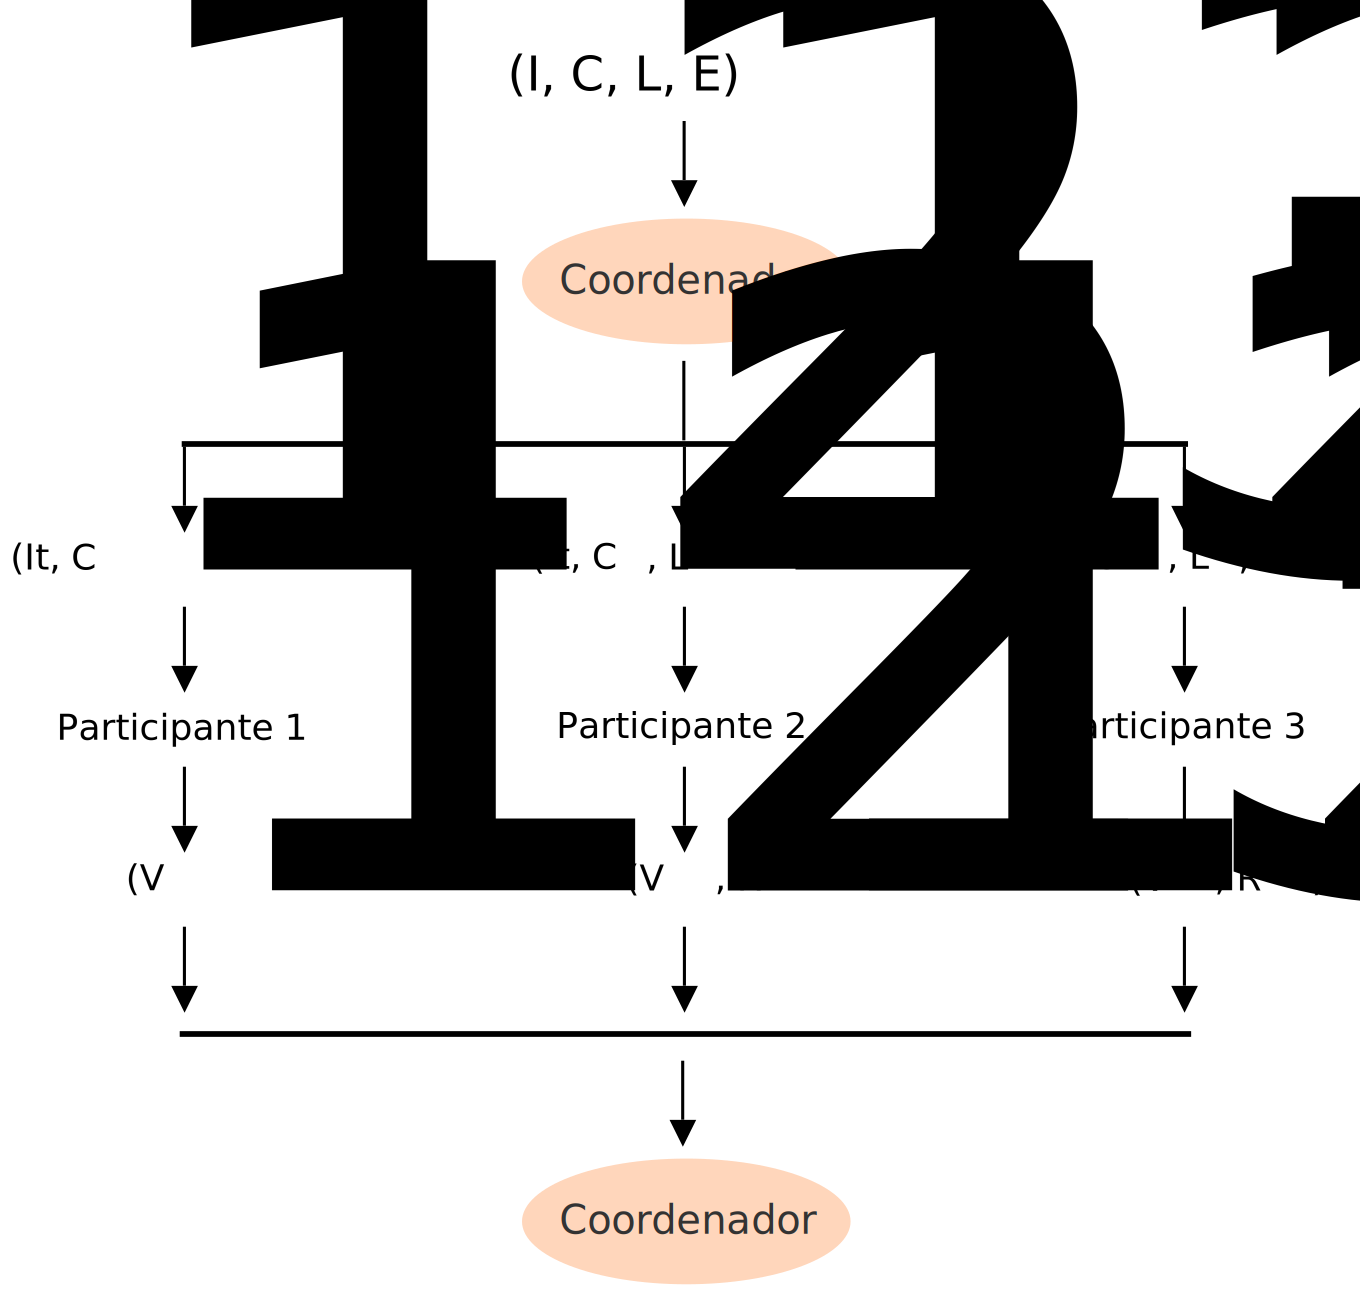
\includegraphics[width=.65\textwidth]{minitransacao_1fase} 
  \caption{Fase de execução de uma minitransação}
  \label{fig:minitransacao_1fase} 
\end{figure}

Se a comparação for bem sucedida para todos os elementos de $Id[C_j]$, então o participante irá ler os dados identificados por $L_J$ e agrupá-los no conjunto de resposta $R_j$. Os dados $Dado[E_j]$ identificados por $Id[E_j]$ serão inseridos no conjunto de dados ou irão alterar algum dado já existente. Na verdade, a operação de inserir ou alterar um dado é registrada no \emph{log} do participante. O participante envia então um voto $EFETIVAR$ para o coordenador, junto com o conjunto $R_j$. 

Ao coletar todas as respostas, o coordenador irá apurar os votos de cada participante. Para cada resposta $EFETIVAR$ o coordenador agrega os respectivos $R_j$ em um conjunto de respostas $R$. Se uma das respostas for $ABORTAR$, a transação precisa ser abortada, notificando os participantes do cancelamento, e a aplicação cliente precisa ser notificada desse erro, como podemos ver na Figura \ref{fig:minitransacao_2fase} \textbf{b}. Se não houve nenhum voto $ABORTAR$, o coordenador decide então por efetivar a transação, enviando o conjunto $R$ para a aplicação cliente e notificando os participantes da efetivação, como ilustrado na Figura \ref{fig:minitransacao_2fase} \textbf{a}.

\begin{figure}
  \centering
  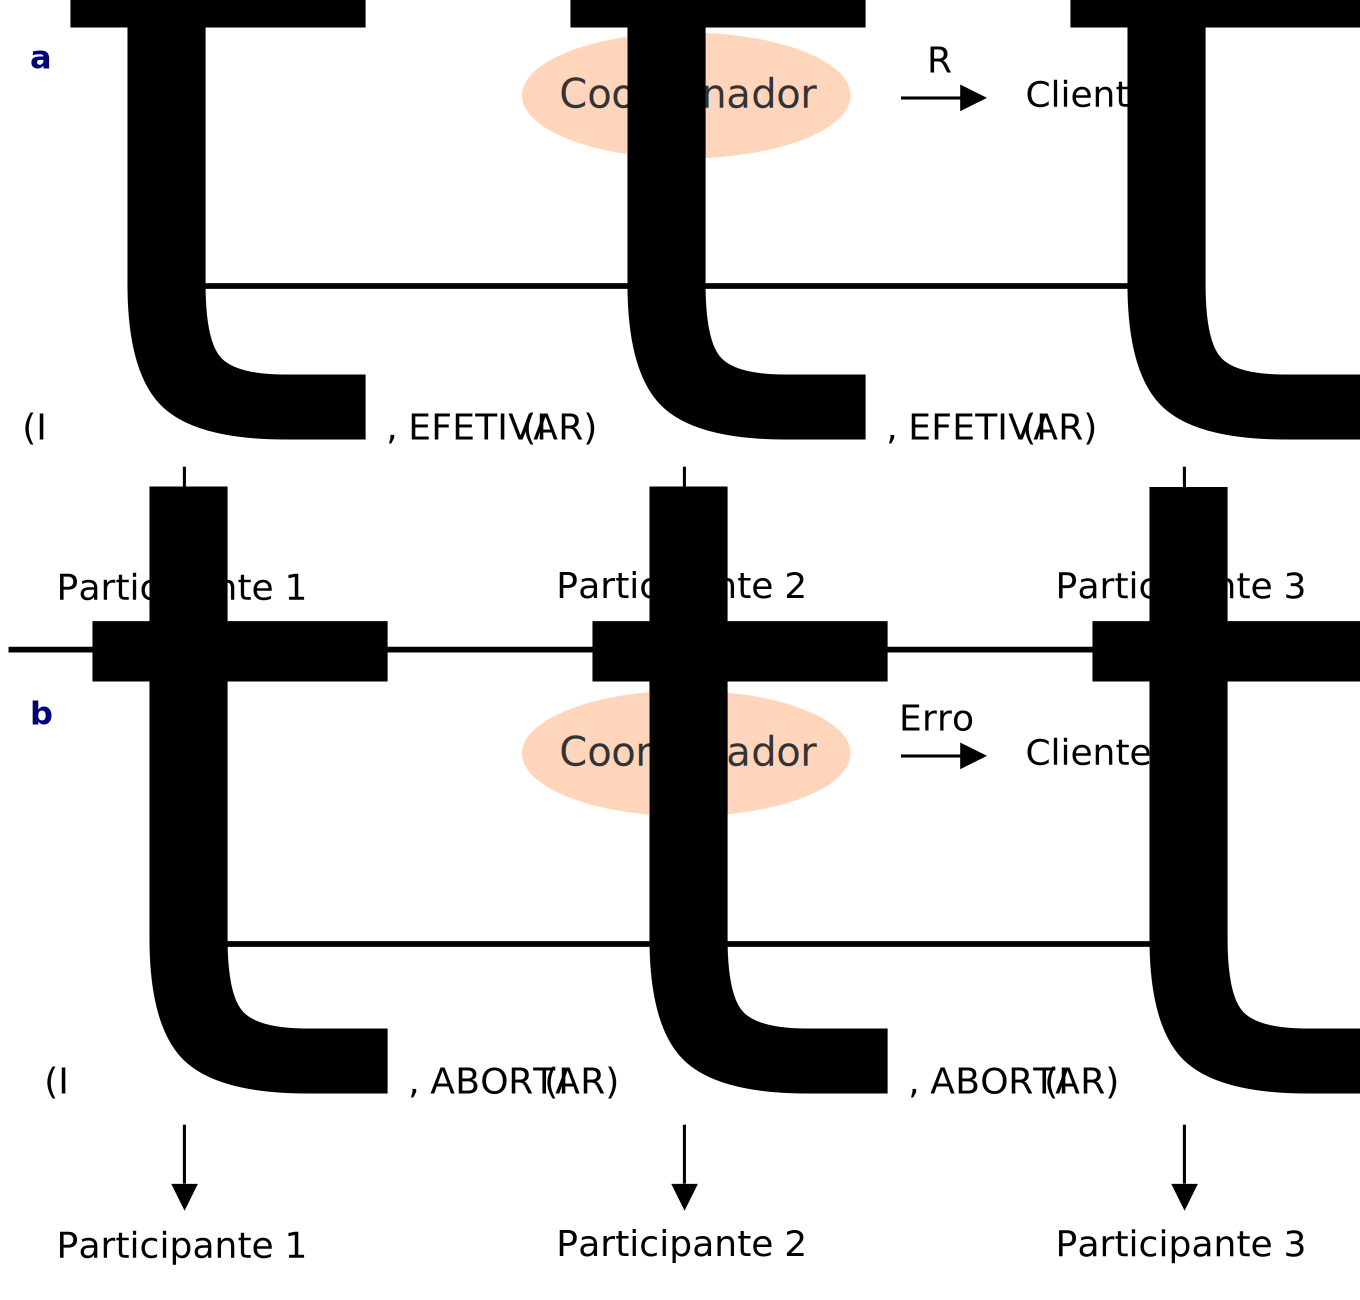
\includegraphics[width=.65\textwidth]{minitransacao_2fase} 
  \caption{Fase de notificação de uma minitransação}
  \label{fig:minitransacao_2fase} 
\end{figure}

Quando os participantes são notificados do cancelamento da minitransação, as operações de escrita da minitransação presentes no \emph{log} do participante não serão efetuadas, deixando os dados inalterados, e será registrado no \emph{log} que a minitransação foi abortada. Se a notificação for de efetivação, as operações de escrita do \emph{log} serão efetuadas, alterando dados existentes ou inserindo novos dados no participante, e será registrado no \emph{log} que a minitransação foi efetivada. O \emph{log} será gravado em disco e a minitransação será considerada oficialmente efetivada ou abortada no momento que esse registro do \emph{log} estiver gravado em disco.

\section{Trabalhos relacionados}
\label{sec:trabalhos_relacionados}
O conceito de minitransações é introduzido como base para a construção de \emph{Sinfonia} \cite{sinfonia}, um sistema cujo foco é prover a base para o desenvolvimento de sistemas distribuídos de baixo nível, como sistemas de arquivos distribuídos, gerenciadores de travas ou serviços de comunicação de grupos de computadores, enquanto que o objetivo deste trabalho é utilizar as minitransações como base para a construção de uma infraestrutura que facilite o desenvolvimento de aplicações distribuídas de alto nível, como sistemas de comércio eletrônico ou redes sociais.

\cite{padilha} apresenta um sistema de armazenamento baseado em minitransações tolerante a falhas bizantinas. Em sistemas que toleram somente componentes com falhas simples (\emph{fail-stop components}), é assumido que um componente pode estar em dois estados: ativo e inativo. Se estiver em um estado ativo, o componente se comportará de acordo com a especificação do sistema. Se estiver inativo, o componente simplesmente para de interagir com o sistema. Essa é uma maneira simples e um tanto simplificada de lidar com falhas no sistema, mas é a forma utilizada por diversos sistemas, entre eles \emph{Sinfonia} e a nossa infraestrutura. A maneira mais geral de lidar com falhas é através da modelagem de falhas bizantinas \cite{byzantine}. Em sistemas que lidam com esse tipo de falha, um componente ativo pode se comportar de forma incorreta, enviando mensagens com conteúdo aleatório (correto ou incorreto), ou não enviando mensagem nenhuma. O tratamento de falhas bizantinas não será discutido neste trabalho.

O uso mais difundido de transações é no contexto dos gerenciadores de bancos de dados relacionais, como \emph{Oracle} \cite{oracle}, \emph{MySQL} \cite{mysql}, \emph{SQL Server} \cite{sqlserver}, entre diversos outros. O tipo de transação oferecida por esses sistemas é normalmente chamada de ACID (Atomicidade, Consistência, Isolamento e Durabilidade) \cite{vaca}. Essas transações podem ser usadas em cenários nos quais não conseguimos utilizar as minitransações, sendo portanto muito mais gerais. Porém, devido às propriedades que devem garantir, o uso dessas transações não permite escalar o banco de dados para um grande número de máquinas, algo que as minitransações permitem.

Existem diversos sistemas que visam o armazenamento escalável de informações e a disponibilização de serviços para facilitar o  desenvolvimento de sistemas distribuídos, visando em geral a utilização em aplicações de internet de larga escala. Entre eles, podemos citar \emph{Bigtable} \cite{bigtable}, \emph{Dynamo} \cite{dynamo}, \emph{ZooKeeper} \cite{zookeeper}, e \emph{PNUTS} \cite{pnuts}.

\emph{Bigtable} é o sistema de armazenamento distribuído do \emph{Google} que oferece uma abstração de um mapa ordenado, multidimensional, esparso e distribuído. \emph{Dynamo}, da \emph{Amazon}, é um sistema de armazenamento chave-valor que visa oferecer alta disponibilidade às aplicações. Esses dois sistemas permitem que dados sejam particionados e replicados para obter melhor desempenho e disponibilidade, mas
permitem que diferentes máquinas possam ter versões diferentes de uma mesma informação.

\emph{ZooKeeper} é um sistema que provê serviços de coordenação e sincronização para a construção de sistemas distribuídos que utiliza o algoritmo \emph{Paxos} \cite{paxos} para garantir consistência entre as operações. Como o objetivo do \emph{ZooKeeper} é permitir a coordenação entre componentes de um sistema distribuído, sua capacidade de armazenamento é limitada (em um \emph{megabyte}), e portanto não é utilizável como um repositório de dados geral.

\emph{PNUTS} é o serviço de armazenamento de dados do \emph{Yahoo!} que garante que todas as réplicas de um determinado dado armazenado executam as mesmas alterações, na mesma ordem. PNUTS permite a existência de várias versões de um dado, e oferece uma primitiva \emph{test-and-set-write}, que efetua uma escrita de dados somente se uma determinada versão do dado for encontrada, semelhante ao mecanismo de comparação das minitransações.

Por último, \emph{Hazelcast} \cite{hazelcast} e \emph{Akka} \cite{akka} são ferramentas para o desenvolvimento de sistemas distribuídos que visam eliminar a necessidade de comunicação explícita entre os participantes do sistema, oferecendo abstrações como estruturas de dados
distribuídas ou memória transacional. \emph{Hazelcast} oferece a programas rodando na \emph{JVM Java} implementações distribuídas das coleções da biblioteca padrão (\emph{Collection, Set, List e Map}). \emph{Akka} permite a utilização de memória transacional por \emph{software} (\emph{software transactional memory} ou \emph{STM} \cite{stm}), uma abordagem que emprega o conceito de transação discutido 
neste trabalho em operações de leitura e escrita na memória principal do computador.

\chapter{A infraestrutura}
\label{chap:implementacao}
Na seção \ref{sec:infinispan} apresenta o Infinispan, detalhando os pontos importantes de sua arquitetura e parte central de sua implementação. 

A seção \ref{sec:mt_infinispan} descreve como as minitransações se encaixam na estrutura de transações do Infinispan e as alterações que foram necessárias nessa estrutura para disponibilizar as minitransações.

\section{Infinispan}
\label{sec:infinispan}
O Infinispan foi escolhido como base para o desenvolvimento de nossa infraestrutura por ser uma plataforma e repositório de dados distribuído. Além disso, ele é um sistema de código aberto, escrito em \emph{Java} \cite{java}, projetado para expor uma estrutura de dados altamente concorrente e para obter o melhor desempenho das modernas arquiteturas de múltiplos processadores e múltiplos núcleos, ao mesmo tempo em que oferece funcionalidades de \emph{cache} distribuído.

Na seção \ref{sec:arquitetura_infinispan} descrevemos a arquitetura do Infinispan, e os principais conceitos sobre os quais essa arquitetura se baseia. A seção \ref{sec:implementacao_infinispan} detalha o núcleo de código que habilita os pontos centrais dessa arquitetura.

\subsection{Arquitetura}
\label{sec:arquitetura_infinispan}
As máquinas rodando Infinispan podem formar um ou mais agrupamentos (\emph{cluster}), caso sejam configuradas de tal forma. Esses agrupamentos permitem que os dados sejam espalhados por diferentes máquinas, permitindo assim uma melhor distribuição de carga entre as máquinas e aumento na disponibilidade dos dados.

O componente principal do Infinispan é a interface \emph{org.infinispan.Cache}, uma extensão da interface \emph{java.util.Map} da biblioteca padrão de coleções do \emph{Java}. O acesso aos dados segue então a mesma abordagem, armazenando entradas, em que um valor é associado a uma chave arbitrária definida pela aplicação. \emph{Cache} permite abstrair os diversos modos de execução em que o Infinispan pode rodar, oferecendo uma interface simples e de ampla utilização para acessar os dados.

Os quatro modos de execução oferecidos pelo Infinispan são:

\begin{description}
	\item[Local] Todas as entradas são armazenadas na máquina local, mesmo que um agrupamento tenha sido formado.
	\item[Replicado] Todas as entradas são copiadas para todas as outras máquinas do agrupamento.
	\item[Distribuído] Cada entrada é replicada para um subconjunto das máquinas do agrupamento.
\end{description}

No modo \textbf{Local} todas as entradas ficam armazenadas na mesma máquina em que o cache está configurado, não permitindo que aplicações compartilhem os dados. O modo \textbf{Replicado} garante alta disponibilidade dos dados, uma vez que cada entrada está copiada em todas as máquinas do agrupamento. Assim, um dado só ficará indisponível no caso em que todas as máquinas do agrupamento em que ele esteja armazenado fiquem indisponíveis. No modo \textbf{Distribuído} o Infinispan armazena uma determinada entrada em um subconjunto do agrupamento. Dessa forma, se esse subconjunto de máquinas ficar indisponível, essa determinada entrada ficará indisponível também. 

O modo \textbf{Distribuído} permite um certo grau de disponibilidade ao mesmo tempo em que oferece um espaço de armazenamento expandido compartilhado entre o agrupamento. Esse grau de disponibilidade é controlado pelo tamanho do subconjunto em que uma entrada será replicada, podendo variar de 1 (não havendo nenhuma replicação, cada entrada é armazenada em somente uma máquina) até o total de máquinas no agrupamento (o que fará esse modo idêntico ao \textbf{Replicado}). O grau de expansão do espaço de armazenamento é inversamente proporcional à disponibilidade, ou seja, quanto maior a disponibilidade, menor a expansão, pois menos espaço ficará disponível devido ao maior número de cópias de uma entrada.

O Infinispan oferece também duas modalidades de acesso:

\begin{description}
	\item[Embarcado]
	\item[Cliente-Servidor] 
\end{description}

Na modalidade de acesso \textbf{embarcado}, o espaço de armazenamento do Infinispan compartilha a mesma máquina virtual \emph{Java} (e portanto, a mesma memória) que a aplicação. No modo \textbf{cliente-servidor}, uma máquina virtual fica dedicada ao espaço de armazenamento do Infinispan, e a aplicação pode acessar esse espaço por meio de alguns protocolos disponíveis: HTTP, Memcached ou HotRod \cite{infinispan}.

As máquinas que compõem o agrupamento (os nós) formam uma rede \textbf{P2P} (\emph{Peer-to-Peer} ou ponto-a-ponto \cite{p2p}). Em uma rede P2P, cada participante (cada nó rodando o Infinispan) compartilha uma parcela de seus próprios recursos (processador, memória, 
etc...) para oferecer um serviço em conjunto com todos os outros participantes (nesse caso, oferecer uma abstração de cache distribuído).
O ponto central dessa rede P2P é que não há distinção entre os nós. Cada nó pode atuar tanto como um provedor quanto como um solicitante de recursos. Qualquer nó pode receber uma solicitação para armazenar ou recuperar um dado associado a qualquer chave, e essa solicitação será atendida de forma transparente por meio da cooperação entre os nós que compõem a rede.

O que permite essa transparência no acesso e independência de localização é uma abstração conhecida como \textbf{DHT} (\emph{distributed hash table}, ou tabela de espalhamento distribuída \cite{dht}). Em uma DHT, existe um conjunto finito de localizadores, e a cada nó que compõe a rede é atribuída a tutela sobre um determinado subconjunto desses localizadores. A DHT permite então encontrar ou armazenar um par de chave e valor por meio do mapeamento da chave para um determinado localizador, que por sua vez está sob a tutela de um nó da rede.

A associação entre localizadores e um nó é feito por uma função de espalhamento consistente (\emph{consistent hashing} \cite{consistent_hashing}), que é um tipo especial de função de espalhamento (\emph{hash function} \cite{taocp_3}). Como toda função de espalhamento, ela mapeia um conjunto de valores para um índice em um espaço de endereçamento (um localizador) de uma forma que a cada localizador desse espaço sejam mapeados subconjuntos com aproximadamente o mesmo tamanho. A propriedade essencial da função de espalhamento consistente que a torna de grande utilidade em um ambiente distribuído é que, ao contrário dos outros tipos de funções de espalhamento, um pequena alteração no espaço de endereçamento resulta em um número pequeno e limitado de remapeamento, mantendo a maioria dos valores mapeados para os mesmos localizadores.

\subsection{Implementação do Infinispan}
\label{sec:implementacao_infinispan}
Infinispan é implementado integralmente na plataforma java, versão padrão (\emph{SE} ou \emph{Standard Edition}). Dessa forma é possível executar o Infinispan em qualquer sistema operacional e plataforma de máquina que ofereça suporte à essa versão do java. Seu código é aberto e público, o que permitiu sua utilização como base para o desenvolvimento de nossa infraestrutura.

A natureza distribuída do Infinispan exige que os nós se comuniquem por meio da rede, e o Infinispan utiliza o JGroups \cite{jgroups} para isso. JGroups oferece uma camada de abstração sobre a rede permitindo um mecanismo de troca de mensagens confiável entre um ou mais nós de uma só vez, que o Infinispan utiliza para a formação dos agrupamentos e comunicação entre os nós.

A interface Cache é uma extensão da interface \emph{java.util.concurrent.ConcurrentMap}, que por sua vez extende \emph{java.util.Map}. \emph{Map} permite armazenar e recuperar entradas compostas por uma chave e um valor, além de possuir alguns outros comandos úteis, como para verificar se uma determinada chave foi armazenada, ou consultar o número de entradas armazenadas. A interface \emph{ConcurrentMap} introduz alguns comandos úteis para a utilização de um mapa em um ambiente de código concorrente, como um comando para armazenar uma entrada somente se a chave associada não tiver sido mapeada (\emph{putIfAbsent}) ou para trocar o valor de uma entrada baseado em um valor já existente (\emph{replace}). A interface Cache acrescenta as funcionalidades para a representação de um cache distribuído e outras funcionalidades específicas para a manutenção e utilização dos agrupamentos formados no Infinispan.

Infinispan começou a ser desenvolvido em paralelo à especificação da JSR-107 \cite{jsr107}, uma padronização ao acesso de mecanismos de cache em java. Essa especificação define uma interface \emph{javax.cache.Cache} que é muito parecida com a interface Cache do infinispan, mas que não disponibiliza acesso a todos os recursos presentes no infinispan. Assim, para poder adequar e permitir que o infinispan possa ser usado por aplicações acessando caches por meio da JSR-107, foi criado o AdvancedCache, uma interface que estende Cache e permite acessar detalhes específicos do infinispan como adicionar e remover interceptadores, gerenciadores de travas e etc. A interface Cache é compatível com a interface de mesmo nome da JSR-107, enquanto que AdvancedCache acrescenta o que é específico do infinispan.

\emph{CacheImpl} é a classe que implementa AdvancedCache (e portanto, Cache). Ela converte as chamadas das funções da interface em comandos representando as ações a serem executadas, contendo referências e informações necessárias para essa execução. Esses comandos são executados por diferentes tipos de processadores de comandos, cada um responsável por diferentes aspectos que um comando apresenta (como distribuição na rede ou persistência de dados em disco). Os processadores são dispostos em uma sequência configurada, e a execução do comando é composta então pela atuação de cada um desses processadores, um após o outro, seguindo a sequência estabelecida. Esse esquema de execução é baseado em alguns padrões (\emph{design patterns}) bem estabelecidos e de ampla utilização, como \emph{Command}, \emph{Visitor}, \emph{Chain of Responsibility} e \emph{Interceptor} (\cite{design_patterns}, \cite{posa}).

Por exemplo, a operação \emph{Cache.get(Object k)}, que permite recuperar a entrada associada à chave \emph{k}, é transformada no comando \emph{GetKeyValueCommand}. De acordo com a configuração e detalhes específicos de cada cache, a sequência de processadores pode ser ligeiramente diferente, mas os tipos mais representativos de processadores são:

\begin{description} 
	\item[DistributionInterceptor] - Provê funcionalidades básicas para que o cache opere de forma distribuída. Processadores mais específicos como \textbf{TxDistributionInterceptor} e \textbf{NonTxDistributionInterceptor} estendem a classe base e são usados de acordo com a configuração para obter melhor desempenho.
	\item[LockingInterceptor] - Gerencia a aquisição e liberação de travas em chaves ou grupos de chaves. Conforme a configuração, são utilizadas classes mais especializadas como \textbf{OptimisticLockingInterceptor} ou \textbf{PessimisticLockingInterceptor}.
	\item[TxInterceptor] - Responsável por tratar de aspectos transacionais, como registrar o cache como um participante em uma transação distribuída.
	\item[CallInterceptor] - Sempre posicionado como o último processador na sequência, é responsável por invocar a operação específica de cada comando.
\end{description}

Um componente muito importante na execução de um comando é InvocationContext, a interface principal da hierarquia ilustrada na figura \ref{fig:invocation_context}, e a escolha de uma ou outra implementação é determinada em tempo de execução de acordo com a configuração. InvocationContext contém informações como o endereço de origem da execução e as chaves sobre as quais a execução obteve travas. AbstractInvocationContext provê a base necessária para a implementação dos contextos, implementando os métodos definidos em InvocationContext de maneira direta. NonTxInvocationContext é utilizado quando o cache não está configurado para utilizar transações, e SingleKeyNonTxInvocationContext é uma otimização para quando a operação envolve somente uma chave. TxInvocationContext permite acessar a transação associada à execução pode ser de dois tipos: LocalTxInvocationContext ou RemoteTxInvocationContext. A implementação Local é utilizada para operações transacionais que foram iniciadas no mesmo nó que estiver executando a operação, e Remote é utilizada quando a operação tiver sido iniciada em um outro nó. 

\begin{figure}
  \centering
  \includegraphics[width=\textwidth]{invocation_context} 
  \caption{Hierarquia de InvocationContext}
  \label{fig:invocation_context} 
\end{figure}

\section{Minitransações no Infinispan}
\label{sec:mt_infinispan}
O subsistema de transações do Infinispan permite agrupar operações em unidades lógicas de execução, oferecendo uma opção transacional para quem utiliza o cache. A seção \ref{sec:tx_infinispan} detalha o subsistema que gerencia e executa transações dentro do Infinispan. A seção seguinte, \ref{sec:suporte_mt_infinispan}, apresenta as modificações necessárias nesse subsistema para que o Infinispan permita a execução de minitransações.

\subsection{O subsistema de transações do Infinispan}
\label{sec:tx_infinispan}
O Infinispan pode ser configurado para agrupar ou não as operações em transações. Quando configurado para não agrupar, cada operação efetuada no cache é considerada isolada, sem relação com as outras operações. Nessa configuração, cada operação pertence a uma transação distinta, que é iniciada antes da operação ser executada e finalizada após o término da execução da operação.

Quando configurado para agrupar as operações, o Infinispan permite que o usuário defina as operações que formam uma transação, explicitamente iniciando e finalizando uma transação de modo a englobar as operações que precisam ser executadas como uma única operação lógica.

A abstração central do subsistema de transações é CacheTransaction, uma \emph{interface Java} \cite{java} que define os detalhes de uma transação no Infinispan. CacheTransaction é o topo de uma complexa estrutura projetada para atender a diferentes demandas transacionais e permitir a integração com \emph{JTA} (\emph{Java Transaction API} \cite{jta}) e \emph{X/Open XA} (\emph{Extended Architecture} \cite{xa}). Um resumo dessa estrutura é apresentado na figura \ref{fig:subsistema_transacoes}.

\begin{figure}
  \centering
  \includegraphics[width=\textwidth]{subsistema_transacoes} 
  \caption{Resumo do subsistema de transações}
  \label{fig:subsistema_transacoes} 
\end{figure}

LocalTransaction é utilizada na execução de transações iniciadas localmente e RemoteTransaction representa uma transação em execução em um nó A que foi iniciada em um outro nó B do agrupamento e que altera informações sob a responsabilidade de A. A classe LocalTransaction referencia uma Transaction do JTA. SyncLocalTransaction é utilizada por SynchronizationAdapter, que implementa a interface Synchronization definida pela JTA. LocalXATransaction é utilizada pelo TransactionXAAdapter, que implementa XAResource para integração com gerenciadores compatíveis com XOpen/XA. Tanto SynchronizationAdapter quando TransactionXAAdapter mapeiam chamadas do JTA e XOpen/XA, respectivamente, para operações de TransactionCoordinator, que centraliza a lógica para o controle de estado e execução das transações. O relacionamento entre essas classes pode ser visto na figura \ref{fig:transaction_coordinator}

\begin{figure}
  \centering
  \includegraphics[width=\textwidth]{transaction_coordinator} 
  \caption{TransactionCoordinator e seus adaptadores}
  \label{fig:transaction_coordinator} 
\end{figure}

GlobalTransaction representa um identificador de transação único em todo o agrupamento, para distinguir uma transação, independente do nó em que foi originada. Ela também é uma representação de alto-nível, sendo especializada por outras classes dependendendo da configuração do Infinispan. A figura \ref{fig:global_transaction} nos mostra de maneira simplificada essas classes. A DldGlobalTransaction implementa algoritmos para detecção de impasses (\emph{deadlocks}) na obtenção de travas para a execução das transações. Xid é uma interface que identifica uma transação no XOpen/XA.

\begin{figure}
  \centering
  \includegraphics[width=\textwidth]{global_transaction} 
  \caption{GlobalTransaction}
  \label{fig:global_transaction} 
\end{figure}

Os comandos que encapsulam operações diretamente relacionadas a uma transação são PrepareCommand, CommitCommand e RollbackCommand. PrepareCommand registra a transação relacionada na estrutura de dados do Infinispan que controla as transações (TransactionTable). CommitCommand e RollbackCommand marcam nessa mesma tabela que a transação relacionada foi finalizada. Outros compartamentos relacionados à esses comandos são implementados nos interceptadores TxInterceptor e TxDistributionInterceptor. TxInterceptor gerencia os comandos transacionais recebidos de outros nós, e TxDistributionInterceptor distribui comandos dentro da transação (como escrita, leitura, etc) para os nós responsáveis pelas chaves especificadas.

Na Listagem \ref{lst:exemplo_transaction} há um trecho de código que ilustra uma transação que utilizaremos para demonstrar como o Infinispan processa transações. Esse código está incompleto e simplificado por questões de clareza.

\begin{lstlisting}[caption={Transação convencional}, label=lst:exemplo_transaction]
cache.getAdvancedCache().getTransactionManager().begin();
cache.put("CHAVE 1", "VALOR 1");
cache.getAdvancedCache().getTransactionManager().commit();
\end{lstlisting}

A primeira linha instrui o gerenciador de transações (\emph{Transaction Manager}) do JTA a criar uma nova transação (\emph{javax.transaction.Transaction} \cite{jta}) e associá-la com a \emph{thread} de execução atual (\cite{ipc}). 

A segunda linha instrui o cache a inserir um novo elemento. Internamente, a classe CacheImpl irá criar os dois objetos necessários para a execução da operação. Um deles é PutKeyValueCommand, responsável por armazenar na chave especificada o valor fornecido. O outro objeto é LocalTxInvocationContext, que vai representar uma execução transacional iniciada no mesmo nó que executa o comando. 

Após criar o comando e o contexto de execução, o infinispan inicia o processamento do comando, oferecendo a cada interceptador configurado a oportunidade de aplicar sua lógica específica à execução do comando em questão. Os interceptadores mais relevantes na execução do comando de escrita são TxInterceptor, LockingInterceptor e EntryWrappingInterceptor.

TxInterceptor vai criar uma implementação de CacheTransaction e mapeá-la para a Transaction criada pela TransactionManager (associada à thread de execução). Dessa forma, a transação pode ser propagada para outro nós (uma vez que a Transaction do JTA não é propagada) e permite que vários nós executem operações em uma mesma transação. O tipo mais comum de CacheTransaction utilizado é o SyncLocalTransaction, que irá permitir que o TransactionManager notifique o infinispan que uma transação foi finalizada.

LockingInterceptor é responsável por efetuar a trava das chaves relacionadas ao comando. Existem duas implementações desse interceptador: OptimisticLockingInterceptor e PessimisticLockingInterceptor. Optimistic utiliza uma abordagem otimista no processo de travamento, postergando a obtenção da trava para o momento da efetivação da transação. Pessimistic tenta obter as travas no momento da execução do comando.

EntryWrappingInterceptor é responsável por obter as entradas do cache referentes às chaves especificadas no comando e disponibilizá-las no contexto de execução. Essas entradas são encapsuladas por uma classe, MVCCEntry, que permite o multiversionamento dos valores e garante as propriedades ACID da transação.

Por último, CallInterceptor irá executar o método \emph{perform} de PutKeyValueCommand, que por sua vez irá alterar o valor da entrada armazenada no contexto de execução disponibilizado por EntryWrappingInterceptor.

A terceira linha faz com que TransactionManager inicie o processo de efetivação da transação. O infinispan faz uso do mecanismo de notificação de eventos do JTA para ser avisado que a transação foi finalizada. Quando isso acontece, é criado um novo contexto de execução e um novo comando do tipo PrepareCommand. Esse comando representa a primera fase do 2PC, e é responsável por notificar os nós participantes da transação que a transação foi finalizada. 

Esse comando será processado pela mesma cadeia de interceptadores configurada, e os interceptadores mais relevantes para esse execução são TxInterceptor e TxDistributionInterceptor. TxInterceptor fica responsável por registrar como \textbf{preparada} a transação em questão, e TxDistributionInterceptor é o responsável por replicar o comando para os outros nós envolvidos na transação.

O próximo passo dependerá do resultado da execução de PrepareCommand. Se nenhum erro ocorrer, TransactionManager irá então solicitar a efetivação da transação. Caso contrário, a transação será cancelada. No caso de efetivação é criado um CommitCommand e no caso de cancelamento, um RollbackCommand. Os dois comandos resultam em marcar a transação como finalizada, mas CommitCommand faz com que EntryWrappingInterceptor efetive as alterações efetuadas nas entradas, disponibilizando-as para outras transações.

\subsection{Suporte a minitransações}
\label{sec:suporte_mt_infinispan}

O objetivo deste trabalho é implementar uma infraestrutura para o desenvolvimento de sistemas distribuídos baseada em minitransações. Para isso, foram necessárias alterações no código do Infinispan para que esse pudesse suportar a execução de minitransações.

\begin{figure}
  \centering
  \includegraphics[width=\textwidth]{transaction_operations} 
  \caption{Estrutura de classes das minitransações}
  \label{fig:transaction_operations} 
\end{figure}

A primeira alteração foi a criação de uma estrutura para representar uma minitransação, ilustrada na figura \ref{fig:transaction_operations}. Minitransaction é a classe que agrupa as operações que podem ser efetuadas no contexto de uma minitransação. A interface MinitransactionOperation é a base que deve ser implementada por qualquer operação que faça parte de uma minitransação.

A operação mais simples é ReadOperation, que especifica a chave cujo valor associado deve ser retornado. ComparisonOperation vai efetuar uma comparação, designada por ComparisonType, entre um valor especificado pelo usuário e o valor associado à chave no cache. WriteOperation irá armazenar no cache o valor especificado e associá-lo à chave especificada. TransformationOperation é a operação mais flexível, pois permite que o usuário aplique uma função de transformação no valor associado à chave especificada. Essa função de transformação é uma implementação de TransformationCallback.

A listagem \ref{lst:exemplo_minitransaction} contém código utilizando minitransações com funcionalidade equivalente ao código da listagem \ref{lst:exemplo_transaction}, e apresenta os principais elementos presentes ao codificarmos utilizando minitransações.

\begin{lstlisting}[caption={Minitransação}, label=lst:exemplo_minitransaction]
Minitransaction minitransaction = new Minitransaction();
minitransaction.addWrite(new WriteOperation("CHAVE 1", "VALOR 1"));
MinitransactionExecution execution = cache.getAdvancedCache().execute(minitransaction);
\end{lstlisting}

O método \textbf{execute} de AdvancedCache inicia criando uma transação em TransactionManager. Esse passo é necessário pois a execução de minitransações é baseada no subsistema de transações do infinispan, e esse vai exigir a presença de uma transação no contexto de execução.

Como segundo passo, \textbf{execute} cria uma PrepareMinitransactionCommand, referenciando o objeto Minitransaction recebido como parâmetro. Esse comando percorre então a cadeia de interceptadores, sendo tratado em quase todos eles da mesma maneira que um PrepareCommand, com exceção de TxInterceptor.

O papel de TxInterceptor ao interceptar PrepareMinitransactionCommand é popular a tabela de transações com uma nova CacheTransaction associada à Transaction atual, e associar ao comando a GlobalTransaction que vai permitir que a transação seja identificada dentro do agrupamento, quando o comando for replicado para os outros nós envolvidos.

A lógica de execução da minitransação, descrita na seção \ref{subsec:estrutura-minitransacoes}, é implementada no método \textbf{perform} de PrepareMinitransactionCommand. O nó para o qual a minitransação foi submetida - aquele em que o método \textbf{execute} foi executado - será chamado aqui de coordenador, e os demais nós envolvidos - aqueles responsáveis por chaves envolvidas na minitransação - são chamados de participantes. Devido ao caráter não-centralizado do infinispan, qualquer minitransação pode ser submetida a qualquer nó do agrupamento, inclusive um nó que não seja responsável por nenhuma chave envolvida na minitransação. Uma chave está envolvida na minitransação se ela for referenciada por qualquer operação dessa minitransação.

O objeto Minitransaction que originou a execução é repassado para todos os nós envolvidos, mas cada nó executa somente as operações relacionadas às chaves sob sua responsabilidade. A replicação de dados que não serão usados não acarreta grandes problemas de performance, mas é um ajuste que pode ser feito facilmente no futuro.

A arquitetura do infinispan permite que tanto o código do coordenador quanto dos participantes seja centralizado no método \textbf{perform} do comando. Quando esse comando é executado como resultado da submissão da minitransação para o coordenador, o fluxo é simplesmente um encadeamento de chamadas de métodos dentro da mesma JVM, que culminam na execução de \textbf{perform} e na obtenção do resultado dessa execução, um MinitransactionExecution. Quando replicado para os participantes, esse comando é transmitido pela rede, reconstruído em cada participante e inserido no fluxo de execução de comandos, como uma chamada de método comum. O objeto retornado pelo método como resultado de sua execução percorre o caminho inverso, sendo enviado de cada participante de volta para o coordenador.

O primeiro passo na execução é obter acesso exclusivo às chaves envolvidas na transação utilizando o mecanismo de travas do infinispan. Um LockControlCommand é criado e executado na cadeia de interceptadores. Se não for possível travar uma ou mais chaves, ocorrerá um erro e a minitransação será cancelada.

Com as entradas referentes às chaves da minitransação travadas, são executadas todas as comparações referentes ao nó atual. Se alguma delas falhar, a minitransação como um todo deve ser cancelada. Para indicar isso, é utilizado o método \textbf{markAsAborted} de MinitransactionExecution. Se todas as comparações forem bem-sucedidas, ou se não houver nenhuma comparação para o nó atual, o fluxo de execução segue.

As operações de leitura são efetuadas em seguida. Para isso, são criados e executados comandos do tipo GetKeyValueCommand, um para cada chave especificada. O valor retornado pela execução de cada um desses comandos é registrado em MinitransactionExecution, com o método \textbf{addReadKeyValue}.

Após as leituras é a vez das operações de escrita, efetuadas com o comando PutKeyValueCommand. Esses comandos são enviados para a cadeia de interceptadores e segue o mesmo fluxo de execução descrito na seção \ref{sec:tx_infinispan}.

O último tipo de operação a ser efetuado é a transformação, que é representada por TransformCommand e por sua implementação de TransformationCallback. Esse comando é semanticalmente muito semelhante à PutKeyValueCommand no sentido em que ele atribui um valor a uma entrada. A diferença é que esse valor é uma função aplicada sobre o valor já existente na entrada. Essa função é representada pela interface TransformCallback e é implementada de acordo com a necessidade do usuário.

Para o nó participante, \textbf{perform} termina nesse ponto, retornando um MinitransactionExecution que será transmitido pela rede para o coordenador. O nó coordenador precisa agrupar todos os resultados obtidos dos participantes e combiná-los por meio do método \textbf{mergeWith} de MinitransactionExecution. Esse método vai agrupar em um só conjunto os resultados das leituras efetuadas e irá marcar esse resultado combinado como sendo cancelado caso algum dos resultados obtidos tenha sido cancelado.

Esse resultado combinado é retornado pelo coordenador e é utilizado pelo método \textbf{execute} para determinar se a minitransação deve ser efetivada ou não. Se \textbf{isAborted} for verdadeiro, a minitransação deve ser abortada e suas alterações devem ser desfeitas. Caso contrário, as alterações devem ser efetivadas e disponibilizadas para futuras transações. Esse processo de efetivação e cancelamento segue o fluxo normal de efetivação e cancelamento do infinispan, sem passar porém pela fazer de preparação do 2PC.

\chapter{Conclusão}
\label{cap:conclusao}

Embora tenha sido planejado para ser modificado, houve alguns pequenos problemas para alterar o infinispan para executar minitransações. Esses problemas e as lições aprendidas com eles estão descritos na seção \ref{sec:problemas_licoes}. Os resultados obtidos com esse trabalho foram disponibilizados para amplo acesso, e uma breve análise está disponível na seção \ref{sec:resultados}. Na seção \ref{sec:trabalhos_futuros} identificamos alguns pontos que podem ser melhorados no trabalho desenvolvido e possíveis extensões.

\section{Problemas, soluções e resultados}
\label{sec:problemas_licoes}

O principal problema encontrado, e de certa forma ainda não resolvido, está relacionado à avaliação da infraestrutura. Esse problema direcionou o desenvolvimento do trabalho para sua direção atual. Os outros problemas estão relacionados ao desenvolvimento.

Inicialmente, foi desenvolvida uma infraestrutura nova, sem utilizar nenhum código como base, em que o processamento de minitransações estava diretamente embutido no sistema. Essa infraestrutura armazena os dados em memória e oferece uma interface de acesso muito parecida à do infinispan. Embora essa primeira infraestrutura desenvolvida funcione e execute minitransações, foram encontrados alguns empecilhos para avaliá-la.

Em primeiro lugar, não foi encontrado nenhum outro sistema que oferecesse essa funcionalidade de execução de minitransações. Não há sentido em avaliar a infraestrutura isoladamente, pois não há nenhum parâmetro de comparação. A avaliação isolada foi feita mas com caráter funcional, para garantir que a infraestrutura estava de acordo com a especificação proposta e que era possível utilizá-la.

A avaliação pretendida era a comparação dos resultados de performance apresentados pela infraestrutura com outros resultados conhecidos, uma vez que um objetivo indireto desse trabalho é demonstrar a efetividade de minitransações como uma alternativa viável para o desenvolvimento de aplicações distribuídas. Porém, essa análise se mostrou mais complexa do que o esperado, pois os outros sistemas disponíveis com funcionalidades semelhantes já estavam consolidados e testados em ambientes de produção de alta-carga, em alguns casos com anos acumulados em melhorias de performance e desempenho.

Surgiu então a idéia de modificar um sistema já existente, que tivesse funcionalidades semelhantes, de forma que a diferença fosse mínima na implementação dos cenários testados. Após a avaliação de alguns candidatos foi escolhido o Infinispan, pois apresentava a maioria das características desejadas para a infraestrutura e era desenvolvido em Java, linguagem com a qual o autor deste trabalho possui maior experiência.

Iniciou-se então um novo esforço de aprendizado, pois o Infinispan é um sistema complexo, com muitas funcionalidade e altamente configurável. Seu código é bem estruturado e faz uso de diversos padrões, convenções e boas práticas utilizadas no desenvolvimento de sistemas distribuídos, mas mesmo assim não é de nenhuma força um código simples. Foram necessárias diversas execuções, novas linhas de log e muitas sessões de debug para que fossem idêntificados os pontos que precisavam ser alterados. 

Ao estender o infinispan, nossa infraestrutura herdou toda sua funcionalidade, como a replicação e distribuição de dados e capacidade de armazenar os dados em diversas formas de armazenagem, como discos ou bancos de dados. Toda a camada de comunição intra-nós e entre a infraestrutura e os clientes também foi reaproveitada. De certa forma, o ponto principal do trabalho passou a ser permitir que o infinispan executasse minitransações, utilizando seus componentes. Isso, porém, não foi tão simples como esperado.

O infinispan pode atuar tanto no modo transacional quanto não-transacional. Porém, o termo "não-transacional" pode dar a impressão de que não há transações envolvidas, o que não é verdade. O deixa de existir é a transação do JTA e a possibilidade de agrupar operações em uma grande operação lógica, demarcada pela usuário. No modo não-transacional, cada operação individual é envolvida por uma transação, criada antes logo no início da execução do comando e finalizada após o fim de sua execução.

Dessa forma, o conceito de transação permeia particamente todo o infinispan, mesmo em trechos que seriam "não-transacionais". Isso dificultou um pouco a inclusão de suporte a minitransações. Por exemplo, não foi possível fazer com que PrepareMinitransactionCommand fosse uma subclasse de PrepareCommand. Inicialmente havia sido codificado dessa forma, mas havia muitos pontos em que PrepareCommand era tratado e a maioria desses pontos não fazia sentido para uma minitransação.

Um outro problema é que o Infinispan faz uma série de otimizações em relação a transações. Uma delas é tratar uma transação distribuída como sendo de somente uma fase, ou seja, em alguns cenários específicos, que dependem da configuração especificada, o infinispan efetua a efetivação ou cancelamento quando processa PrepareCommand. A configuração necessária para habilitar as minitransações resultavam necessariamente nesses cenários, o que atrapalhava a execução das minitransações.

Foram testadas algumas alternativas para a implementação, mas a solução final acabou sendo a mais simples. Foi criado um novo comando, PrepareMinitransactionCommand, e esse comando recebeu um tratamento separado dos outros comandos relacionados ao controle de transação do infinispan. 



%\section{Avaliação e resultados obtidos}
%\label{sec:resultados}


%Foi necessário

%A própria natureza das minitransações dificulta essa comparação pois como vimos, ela está restrita a alguns tipos de operações, sendo menos genérica do que uma transação convencional. Assim, comparar 


%A prosposta deste trabalho é disponibilizar uma infraestrutura com suporte a minitransações para facilitar o desenvolvimento de aplicações distribuídas, mas não foi encontrado nenhum outro sistema que oferecesse essa funcionalidade.



% Nesse âmbito, não foi encontrado nenhum outro sistema que oferecesse essa capacidade específica de minitransações e portanto, foi é possível compará-lo

%Grande parte do esforço de desenvolvimento foi voltado a entender a base de código do infinispan. O seu código está em sua grande maioria bem estruturado, com cada classes com suas responsabilidades bem definidas. A arquitetura da aplicação também foi bem planejada, e a maneira como conceitos e padrões foram usados para viabilizar a complexa tarefa de esconder uma estrutura de cache distribuída atrás de uma interface amigável ao usuário é uma lição muito importante aprendida.


%A primeira proposta desse trabalho era desenvolver uma infraestrutura totalmente do zero, e dessa forma todo o processamento de minitransações estaria embutido no sistema. Esse sistema chegou a ser desenvolvido e, apesar de ter funcionalidades bem simplificadas, as minitransações eram executadas corretamente e de modo integral, mas ele foi descontinuado por apresentar algumas dificuldades com relação à avaliação do sistema.

%A idéia para avaliar o sistema era de comparar  

%Um empecilho ao uso desse sistema era como compará-lo com outros sistemas. Não foi encontrado nenhum outro sistema com suporte a minitransações, e comp

%\section{Trabalhos futuros}
%\label{sec:trabalhos_futuros}

*** TODO colocar a conclusão

% cabeçalho para os apêndices
\newpage
\renewcommand{\chaptermark}[1]{\markboth{\MakeUppercase{\appendixname\ \thechapter}} {\MakeUppercase{#1}} }
\fancyhead[RE,LO]{}
\appendix
\chapter{Códigos}

Esse apêndice apresenta algumas listagens mais completas de códigos e exemplos de utilização do infinispan.

\label{apx:codigo}
\begin{lstlisting}
public interface FlagContainer {

   boolean hasFlag(Flag o);

   Set<Flag> getFlags();

   void setFlags(Flag... flags);

   void setFlags(Collection<Flag> flags);

   void reset();

}
\end{lstlisting}

% ---------------------------------------------------------------------------- %
\backmatter \singlespacing   % espaçamento simples
\bibliographystyle{alpha-ime}% citação bibliográfica alpha
\bibliography{bibliografia}  % associado ao arquivo: 'bibliografia.bib'

\end{document}
